\begin{figure}[]
	\centering
	\begin{tikzpicture}[scale=\textwidth/\paperwidth]
		\begin{scope}[>=latex, node distance=1, align=center, transform shape]
			\node	(aux1)	[]	{};
			\node[core,	minimum height=95]
					(mis)	[left=of aux1,anchor=north east]	{MIS};
			\node[core]	(ram)	[right=of aux1,anchor=north west, text width=30]	{16 kB RAM};
			\node[perif,text width=60]
					(xcvr)	[left=of mis]	{Transceptor USB};
			\node[interior,	minimum size=60, text width=50]
					(uc)	[above=of aux1]	{8051 Mejorado};			
			\node[perif,
			node distance=2.9]
				(pll)	[left=of uc]	{PLL};		
			\node	(aux2)	[right=of ram.south]{};				
			\node[core,	text width=120]
				(bus)	[right=of aux2,rotate=90,anchor=north west]	{Bus de datos y direcciones};		
			\node[perif]	(i2c)	[right=of bus.south east,anchor=north west]	{I2C};
			\node[perif,text width=30]
				(gpif)	[right=of bus.south west,anchor=south west] {GPIF};
			\node[perif,text width=40]
				(fifo)	[below=of gpif]	{4 kB FIFO};
			\node	(aux3)	[right=of fifo]	{};
			\node	(aux5) 	[left=of ram] {};
			\draw[<->]	(mis) -- (xcvr);
			\draw[<->]	(ram) -- (ram -| mis.east);
			\draw[<->]	(fifo) -- (fifo -| mis.east);
			\draw[<->]	(ram) to (ram -| bus.north);
			\draw[<->]	(uc) to (uc -| bus.north);
			\draw[<-]	(xcvr) to (xcvr |- pll.south);
			\draw[->]	(pll) to (uc);
			\draw[<->]	(i2c) to (i2c -| bus.south);
			\draw[<->]	(gpif) to (gpif -| bus.south);
			\draw[]		(fifo) -| (aux5.center);
		\end{scope}
	
		\begin{scope}[on background layer]
			\node[contenedor] (fx2) [fit=(pll)(xcvr)(uc)(bus)(mis)(ram)(fifo)(gpif)(i2c)(aux3)]{};
		\end{scope}
		
		\begin{scope}[transform shape,>=latex]
			\node[text width=40,align=center]	(xtal)	[left=of pll]{Xtal \SI{24}{\mega\hertz}};
			\node	(host)	[left=3of xcvr]	{PC};
			\draw[<->,ultra thick] (host) -- node [above,text width=70,midway,align=center]{Comunicación USB} (xcvr);
			\draw[->] (xtal) to (pll);
			\draw[<->,ultra thick] (bus.240) -- node [above,align=center,text width=80] {Datos, direcciones y entradas adicionales}(bus.240 -| fx2.east);
			\draw[<->,thick] (gpif) to (gpif -| fx2.east);
			\draw[<->,thick] (fifo) to (fifo -| fx2.east);
			\draw[<->,thick] (i2c) to (i2c -| fx2.east);
		\end{scope}
	\end{tikzpicture}
	%		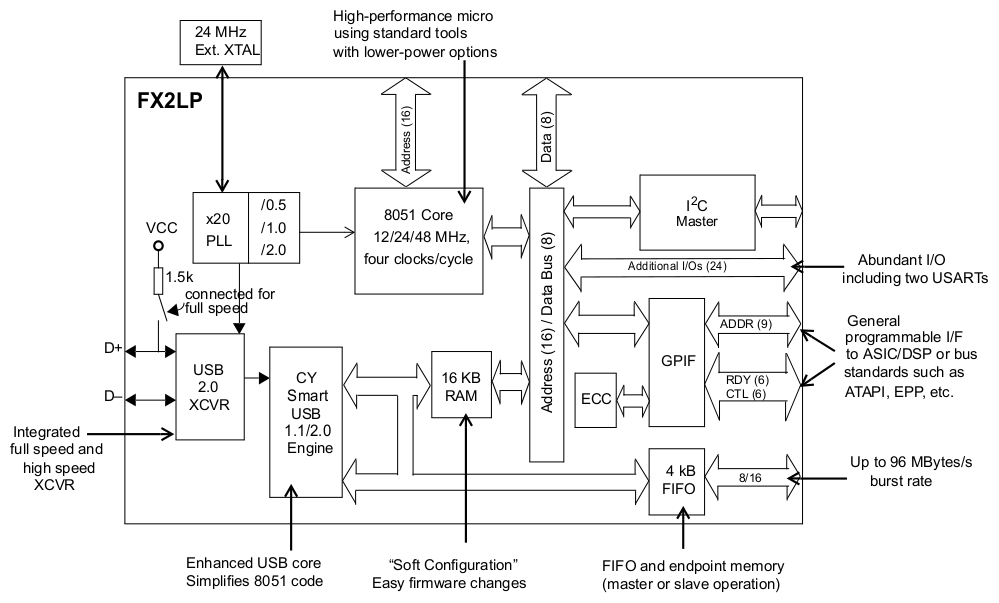
\includegraphics[width=.7\textwidth]{arqfx2lp.png}
	%		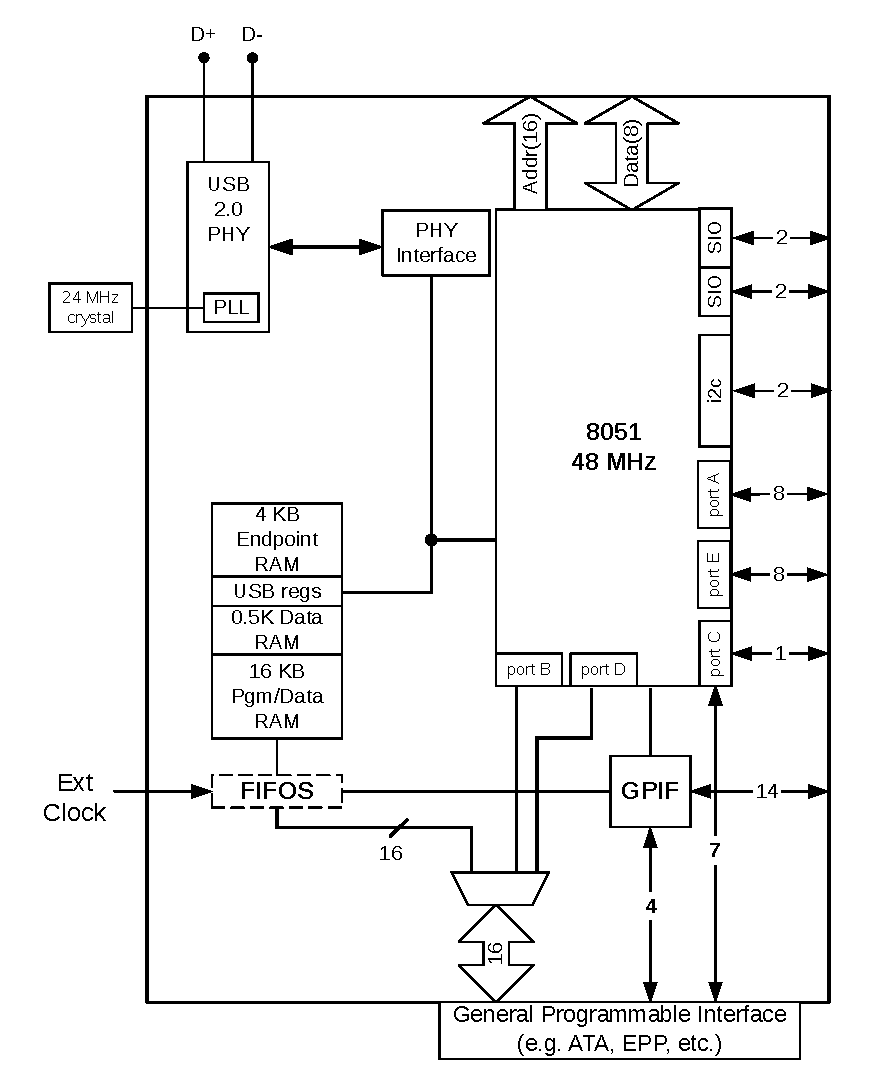
\includegraphics[width=.55\textwidth]{arq.eps}
	\caption{Arquitectura FX2LP} 
	\label{arqEzUSB}
\end{figure}

El núcleo del Kit de Desarrollo CY3684 es el controlador EZ-USB FX2LP. La serie de controladores FX2LP se caracteriza por brindar una conexión USB 2.0 de alta velocidad y bajo consumo energético. Está diseñada, preferentemente más no exclusivamente, para periféricos con autonomía limitada.

La arquitectura de controlador FX2LP, tal como se presenta en la Figura \ref{arqEzUSB}, integra un controlador USB completo. Incluye un transceptor USB, un Motor de Interfaz Serie (MIS), buffers de datos configurables, un microcontrolador 8051 que contiene registros y funciones adicionales orientadas a mejorar el rendimiento de la comunicación USB y una interfaz programable hacia los periféricos implementada con memoria tipo FIFO (\(First In First Out\); Primero Entrado, Primero Salido). Además posee un PLL con divisor configurable a través del cual provee las señales de reloj adecuadas para el correcto funcionamiento del sistema.%\\

El flujo de datos posee dos puntas (una PC y un FPGA) entre las cuales el controlador cumple el rol de interfaz. Para ello necesita poder comunicarse tanto con el host como con los periféricos. El usuario puede trasmitir datos desde y hacia el host a través del mismo puerto USB. Sin embargo, también posee dos puertos DE-9 que permiten comunicarse con la PC a través del protocolo UART (acrónimo de Transmisión y Recepción Asíncrona Universal, en inglés) que facilitan en gran medida la tarea de depuración del desarrollo gracias a que posee una configuración simple.

En cuanto a la interfaz con uno o mas perifericos, el controlador posee un puerto $I^2C$, una interfaz de propósito general (GPIF), para sistemas que necesitan ser comandados en forma externa; y una interfaz con memorias FIFO esclavas, a través de las cuales se puede conectar sistemas que cumplen un rol activo en el envío y recepción de información. Estas tres interfaces posibilitan la conexión de dispositivos que poseen tanto puertos estandarizados (ATA, PCMCIA, EPP, etc.), cómo personalizables (DSP, FPGA, microcontroladores, etc).

%Variante 1
 
%El usuario puede trasmitir datos desde y hacia el anfitrión a través del mismo puerto USB, o bien via RS-232. Para comunicarse con sistemas periféricos se puede aprovechar el puerto $I^2C$, la interfaz de propósito general, que actúa como maestro y a la cual se le puede acoplar un periférico esclavo, y/o las memorias FIFO en modo esclavo que puede ser conectada a un sistema maestro. Esto brinda muchas alternativas, desde la conexión a puertos estandar, como ser ATA, PCMCIA, EPP, etc. o también la conexión de dispositivos tales como DSP's y FPGA's.\\
%\textbf{\hl{variante 1}}
%\hl{El usuario puede trasmitir datos desde y hacia el anfitrion a traves del mismo puerto USB, o bien via RS-232. Para comunicarse con sistemas perifericos se puede aprovechar el puerto $I^2C$, la interfaz de proposito general, que actua como maestro y a la cual se le puede acoplar un periferico esclavo, y/o las memorias FIFO en modo esclavo que puede ser conectada a un sistema maestro. Esto brinda muchas alternativas de conexion, desde puertos estandar, como ser ATA, PCMCIA, EPP, etc. hasta dispositivos personalizables como DSP's y FPGA's}.%\\

%variante 2
%El flujo de datos posee dos puntas entre las cuales el controlador hace de nexo. Para ello necesita poder comunicarse tanto con el \host como con los periféricos.\\
%
%El intercambio de información con el \host se lleva a cabo a través del mismo puerto USB, objetivo principal de este trabajo. Sin embargo, también posee dos puertos UART que facilitan en gran medida la tarea de depuración del desarrollo.\\
%
%En cuanto a la interfaz con uno o más periféricos, el controlador posee un puerto $I^2C$, una interfaz de propósito general (GPIF), para sistemas que necesitan ser comandados en forma externa; y una interfaz con memorias FIFO esclavas, a través de las cuales se puede conectar sistemas que cumplen un rol activo en el envío y recepción de información.\\

%\textbf{\hl{variante 2}}
%
%\hl{El flujo de datos posee dos puntas (una PC y un FPGA) entre las cuales el controlador cumple el rol de interfaz. Para ello necesita poder comunicarse tanto con el host como con los perifericos.}%\\
%
%\hl{El intercambio de informacion con el HOST se lleva a cabo a traves del mismo puerto USB, objetivo principal de este trabajo. Sin embargo, tambien posee dos puertos UART que facilitan en gran medida la tarea de depuracion del desarrollo.}%\\
%
%\hl{En cuanto a la interfaz con uno o mas perifericos, el controlador posee un puerto $I^2C$, una interfaz de proposito general (GPIF), para sistemas que necesitan ser comandados en forma externa; y una interfaz con memorias FIFO esclavas, a traves de las cuales se puede conectar sistemas que cumplen un rol activo en el envio y recepcion de informacion.}%\\

Este trabajo utiliza particularmente las memorias FIFO en modo esclavo, que responden a las diferentes señales que les proporciona un maestro externo implementado con un FPGA; por lo que a continuación se explicitan algunos detalles referidos a ellos, con lo que se busca aclarar el funcionamiento y que el lector comprenda los fundamentos de las configuraciones que se plasman en el código del firmware.

\subsection{Motor de Interfaz Serial}
	El Motor de Interfaz Serial (MIS) es un módulo incorporado al circuito integrado que se encarga de tomar datos en paralelo y convertilos en una secuencia seriada.

	\begin{figure}[ht]%TODO hacer con tikz para que quede prolija
		\centering
		\includegraphics[width=.8\textwidth]{usbxcvr}
		\caption{Implementación del enlace USB realizado por el EZ-USB (\hl{se copiaria con tikz para mejorar prolijidad})}
		\label{usbxcvr}
	\end{figure}
	
	La comunicación USB entre el controlador FX2LP y la PC se realiza a través del transceptor, unido al MIS. Con el objetivo de intercambiar datos, el firmware solo debe colocar o extraer los datos de buffers programables y modificar las banderas de handshaking. En forma automática, el MIS se encargan de empaquetar, enviar, recibir y desempaquetar toda la información, así como leer los tokens que emite el host, calcular y corroborar los códigos cíclicos de detección de errores y todo lo relacionado al protocolo propiamente dicho. El transceptor codifica y decodifica todo a nivel físico.%\\
	
	La Figura \ref{usbxcvr} muestra la función del MIS. Toma los datos colocados en los buffers de extremos, agrega la información que corresponde al encabezado y a la cola y, finalmente, coloca el registro de handshaking. Esto último, se observan como ACK (abreviación del ingles {\it acknowledge}, que significa reconocer, aceptar o agradecer) en la Figura \ref{usbxcvr}. En el extremo del controlador, estas banderas se colocan en un registro especial que indica si el sistema está disponible, si los datos fueron colocados o leídos, dependiendo el caso tratado.
		
\subsection{Buffers de extremos}
	El MIS guarda los datos que aún no han sido enviados y/o los que han sido recibidos pero no leídos por ningún periférico en una memoria RAM específica, denominada buffer de extremo.%\\
	
	La norma USB define a un dispositivo extremo como una porción exclusiva e identificable de una dispositivo USB que es fuente o un sumidero de información. En otras palabras, USB ve a cada extremo como una memoria FIFO de donde surge o finaliza la información. En ingles, el termino extremo recibe el nombre de {\it endpoint}, por lo que, en adelante, cuando se hable de ellos se abreviara como EP o EPx, siendo la x un número que indica la dirección del extremo.%\\
	
	La serie de controladores FX2LP dispone de hasta 7 EP programables, los cuales deben poseer al menos dos buffers. La norma USB indica que cualquier dispositivo USB debe poseer un EP con dirección 0 que se destina para control y configuración, por lo que el controlador está dotado de \SI{64}{\byte} para este fin. Es el único EP que puede ser bidireccional en el sentido del flujo de datos. A través de él, \host y dispositivo intercambiarán solo transferencias de control. Luego, se incorpora un EP1, que posee dos buffers fijos, o sea no configurables, de 64 bytes, uno como entrada y el otro como salida.%\\
	
	\begin{figure}[t]
		\centering
		\begin{tikzpicture}[scale=.7*\textwidth/\paperwidth,node distance=2.7]
			\begin{scope}[transform shape]
				\begin{scope}[node distance=0.4]
					\node[buf]	(ep2b1)	[anchor=north]		{\ep{1}{2}{512}};
					\node[buf]	(ep2b2)	[below=of ep2b1]	{\ep{2}{2}{512}};
					\node[obuf]	(ep4b1) [below=of ep2b2]	{\ep{1}{4}{512}};
					\node[buf]	(ep4b2) [below=of ep4b1]	{\ep{2}{4}{512}};
					\node[obuf]	(ep6b1)	[below=of ep4b2]	{\ep{1}{6}{512}};
					\node[buf]	(ep6b2)	[below=of ep6b1]	{\ep{2}{6}{512}};
					\node[obuf]	(ep8b1)	[below=of ep6b2]	{\ep{1}{8}{512}};
					\node[buf]	(ep8b2)	[below=of ep8b1]	{\ep{2}{8}{512}};
				\end{scope}
				
				\begin{scope}[node distance=0.4, xshift=90]
					\node[buf]	(ep2b3)	[anchor=north]		{\epg{1}{2}{1024}};
					\node[obuf] (ep2b4)	[below=of ep2b3]	{\epg{2}{2}{1024}};
					\node[obuf]	(ep2b5)	[below=of ep2b4]	{\epg{3}{2}{1024}};
					\node[obuf]	(ep8b3)	[below=of ep2b5]	{\ep{1}{8}{512}};
					\node[buf]	(ep8b4)	[below=of ep8b3]	{\ep{2}{8}{512}};
				\end{scope}
			\end{scope}
		
			\begin{scope}[on background layer]
				rounded corners,]
				\node[env, fit=(ep2b1)(ep2b2)]			(ep21)	{};
				\node[env, fit=(ep4b1)(ep4b2)]			(ep41)	{};
				\node[env, fit=(ep6b1)(ep6b2)]			(ep61)	{};
				\node[env, fit=(ep8b1)(ep8b2)]			(ep81)	{};
				\node[env, fit=(ep2b3)(ep2b4)(ep2b5)]	(ep22)	{};
				\node[env, fit=(ep8b3)(ep8b4)]			(ep82)	{};
				\node[draw=black,fit=(ep21)(ep82)](marco){};
			\end{scope}
		
			\begin{scope}[transform shape]
				\draw (marco.north) to (marco.south);
				\node[left=of ep2b1.north east,anchor=north east](add1)	{0xF000};
				\node[left=of ep2b1.south east,anchor=south east](add2)	{0xF1FF};
				\node[left=of ep2b2.north east,anchor=north east](add3)	{0xF200};
				\node[left=of ep4b1.north east,anchor=north east](add4)	{0xF400};
				\node[left=of ep6b1.north east,anchor=north east](add5)	{0xF800};
				\node[left=of ep8b1.north east,anchor=north east](add6)	{0xFC00};
				\node[left=of ep8b2.south east,anchor=south east](add7)	{0xFFFF};
				\draw[dashed] (add1.north west) to (add1.north west -| marco.east);
				\draw[dashed] (add3.north west) to (add3.north west -| ep21.east);
				\draw[dashed] (add4.north west) to (add4.north west -| marco.east);
				\draw[dashed] (add5.north west) to (add5.north west -| marco.east);
				\draw[dashed] (add6.north west) to (add6.north west -| marco.east);
				\draw[dashed] (add7.south west) to (add7.south west -| marco.east);
			\end{scope}
	\end{tikzpicture}
	\caption{Buffers de extremos con sus direcciones de memoria. El cuadro de la izquierda muestra la configuración por defecto. El derecho, la implementada en este trabajo.}
	\label{epbuf}
	\end{figure}
	
	Finalmente, se incorpora una memoria de \SI{4}{\kibi\byte} que debe ser configurada para los EP2, EP4, EP6 y EP8. La configuración de los EP la realiza el microcontrolador una vez que su programa se encuentra en ejecución. Las variables, conforme a los requerimientos de ancho de banda y acceso al bus son:
	
	\begin{itemize}
		\item Tamaño: Dependiendo del extremo a configurar puede ser de 512 o 1024 bytes.
		\item Tipo de acceso al bus: Definido según la norma USB, este tipo puede ser por bultos, isocrónico o de interrupción. No se admiten en estos EP paquetes de control.
		\item Cantidad de buffers: Dependiendo del extremo, puede ser dos, tres o cuatro buffers por extremo.
		\item Habilitación: Se debe indicar al sistema si los extremos se usan o no. El EP no valido, no responderá a un pedido de entrada o salida.
	\end{itemize}
	
	La Figura \ref{epbuf} muestra solo dos de las posibles configuraciones de los EP. A la izquierda se observa la configuración por defecto del controlador FX2LP. Esto es, los cuatro EP habilitados, con 512 bytes cada uno, buffers dobles y comunicación por bultos. A la derecha se muestra la configuración elegida para este trabajo, es decir, solo son EP válidos el EP2 y EP8. EP2 posee tres buffers de 1024 bytes y el EP8 dos buffers con 512 bytes de capacidad cada uno. Siempre se debe considerar que se dispone hasta \SI{4}{\kibi\byte} de memoria.%\\
	
	La característica de los buffers múltiples evita la congestión de datos. Con doble buffer, un periférico (o el microcontrolador) coloca o extrae datos de un buffer, mientras otro, del mismo EP, se encuentra enviando o recibiendo datos mediante el MIS. Cuando se configura un triple o cuádruple buffer, se agrega una o dos porciones mas de memoria a la reserva, respectivamente. De esta forma, se le otorga al sistema una gran capacidad de datos y ancho de banda.%\\
	
	Un detalle importante de los buffers múltiples es que, a la vista del controlador y/o de un periférico, el buffer posee una sola y única dirección y, es la propia interfaz FX2LP quien se encarga de seleccionar el buffer que corresponde en cada caso. Esto quiere decir que, por ejemplo, teniendo 4 buffers de 512 bytes cada uno, el 8051 verá solo uno de 512 bytes, sin necesidad de identificar a traves de su firmware con cuál de los cuatro está trabajando.
	
\subsection{Memorias FIFO esclavas}		

	Desde un punto de vista digital, el MIS recibe y envía datos desde y hacia el puerto USB. Para ello utiliza un cristal de \SI{24}{\mega\hertz}. Por su parte, un sistema externo puede o no proveer una señal de reloj y manejo de datos propio. El controlador USB incorpora memorias FIFO que se encargan de proveer una interfaz entre el MIS y un dispositivo externo, salvando el problema de poseer dos relojes diferentes e independientes.%\\
	
	Estas memorias funcionan en modo esclavo, es decir, se debe conectar un dispositivo capaz de proveer una lógica maestra externa que comande la entrada y salida de datos desde una memoria FIFO hacia o desde el exterior. Para los fines del presente trabajo, este modo de funcionamiento es óptimo ya que, dotando al FPGA de una máquina de estados, se logra la transferencia de datos en los tiempos requeridos.%\\
	
	El sistema de bus permite conectar a estas memorias hasta cuatro dispositivos diferentes. Por esto, existe un registro que permite seleccionar una porción de memoria FIFO para cada uno de los EP programables en el buffer de extremos.%\\
	
	\begin{figure}[ht]
		\centering
		\begin{tikzpicture}[scale=1*\textwidth/\paperwidth]
			\begin{scope}[transform shape,node distance=4,>=latex]
				\node[simple]	(fifo)		[]	 			{FIFO's Esclavas};
				\node[simple]	(master)	[right=of fifo]	{Maestro Externo};
				\draw[<->,thick]	([yshift=5*110/6]fifo.east) --node [above]{IFCLK} ([yshift=5*110/6]master.west);
				\draw[<->,thick]	([yshift=4*110/6]fifo.east) --node [above]{FD[15:0]} ([yshift=4*110/6]master.west);
				\draw[<-,thick]	([yshift=3*110/6]fifo.east) --node [above]{FIFOADR[1:0]} ([yshift=3*110/6]master.west);
				\draw[->,thick]	([yshift=2*110/6]fifo.east) --node [above]{FLAGA} ([yshift=2*110/6]master.west);
				\draw[->,thick]	([yshift=1*110/6]fifo.east) --node [above]{FLAGB} ([yshift=1*110/6]master.west);
				\draw[->,thick]	([yshift=0*110/6]fifo.east) --node [above]{FLAGC} ([yshift=0*110/6]master.west);
				\draw[->,thick]	([yshift=-1*110/6]fifo.east) --node [above]{FLAGD} ([yshift=-1*110/6]master.west);
				\draw[<-,thick]	([yshift=-2*110/6]fifo.east) --node [above]{SLOE} ([yshift=-2*110/6]master.west);
				\draw[<-,thick]	([yshift=-3*110/6]fifo.east) --node [above]{SLWR} ([yshift=-3*110/6]master.west);
				\draw[<-,thick]	([yshift=-4*110/6]fifo.east) --node [above]{SLRD} ([yshift=-4*110/6]master.west);
				\draw[<-,thick]	([yshift=-5*110/6]fifo.east) --node [above]{PKTEND} ([yshift=-5*110/6]master.west);
			\end{scope}				
		\end{tikzpicture}
		\caption{Puertos de interfaz entre las FIFO's y un maestro externo}
		\label{interfazfifo}
	\end{figure}

	La Figura \ref{interfazfifo} muestra las señales de la interfaz entre las memorias FIFO's y un maestro esclavo. Estas son:
	
	\begin{itemize}
		\item IFCLK: señal de reloj. No es necesario en caso de conectar la interfaz en modo asincrónico. La señal de reloj puede ser provista por el controlador o por el dispositivo de control en forma programable.
		\item FD[15:0]: constituye el bus de datos. Según se programe, este puede ser de 8 o 16 bits, en forma independiente para cada EP.
		\item FIFOADDR[1:0]: puerto de direcciones. A través de el se selecciona la memoria activa en el bus.
		\item FLAGx: Los cuatro puertos de flag son configurables e indican memoria llena, vacía o un nivel programable. También pueden indicar el estado sobre una memoria en particular o sobre la activa.
		\item SLOE, SLWR, SLRD: son las señales de control. A través de ellas el maestro entrega las ordenes de lectura y escritura.
		\item PKTEND: a través de este puerto el maestro indica que terminó una transferencia de datos.
	\end{itemize}

\subsection{Modos de entrada y salida automáticos}
	\begin{figure}[ht]
		\centering
		\begin{tikzpicture}[scale=0.8\textwidth/\paperwidth,text width=5em,align=center,>=latex,node distance=31mm]		
		\begin{scope}[transform shape]
		\node[interior]	(mis)									{MIS};
		\node			(im)	[right=of mis]					{};
		\node[interior]	(uc)	[above=of im]					{$\mu$C};
		\node[interior] (fifo)	[right=of im,text width=4em]	{FIFOs Esclavas};
		\node			(et)	[left=of uc]					{FX2LP};
		
		\draw[->]([xshift=1.5mm]fifo.north)to node[above,mode text]{MODO ENTRADA MANUAL} ([yshift=1mm]uc.east);
		\draw[->]([yshift=1mm]uc.west)to node[above,mode text]{MODO ENTRADA MANUAL}([xshift=-1.5mm]mis.north);
		\draw[->] ([yshift=-1mm]uc.east)to node[below,mode text]{MODO SALIDA MANUAL}([xshift=-1.5mm]fifo.north);
		\draw[->]([xshift=1.5mm]mis.north)to node[below,mode text]{MODO SALIDA MANUAL}([yshift=-1mm]uc.west);
		
		\draw[->]([yshift=1mm]fifo.west)to node[above,mode text]{MODO AUTO ENTRADA}([yshift=1mm]mis.east);
		\draw[->]([yshift=-1mm]mis.east)to node[below,mode text]{MODO AUTO SALIDA}([yshift=-1mm]fifo.west);
		
		\node[exterior]	(pc)	[left=of mis]	{Host};
		\draw[->]([yshift=1mm]mis.west)to([yshift=1mm]pc.east);
		\draw[->]([yshift=-1mm]pc.east)to([yshift=-1mm]mis.west);
		
		\node[exterior]	(fpga)	[right=of fifo]	{Maestro Externo};
		\draw[->]([yshift=1mm]fifo.east)to node[above]{Banderas}([yshift=1mm]fpga.west);
		\draw[<-]([yshift=-1mm]fifo.east)to node[below]{Control}([yshift=-1mm]fpga.west);
		\end{scope}	
		
		\begin{scope}[on background layer]
		\node(fx)[rounded corners,fill=black!10,fit=(mis)(uc)(fifo)(et)]{};
		\end{scope}
		\end{tikzpicture}
		\caption{Modos de conexión de la memoria FIFO, el microntrolador y el MIS}
		\label{modesfifo}
	\end{figure}

	
	Los datos que se reciben o envían a través del MIS. Pueden ser enviados en forma automática desde y hacia las memorias FIFO, o bien, pueden ser dirigidos a través del microcontrolador. Esto último permite leer, modificar, suprimir, agregar y/o generar nuevos datos antes de ser remitidos como paquete, es decir, todos juntos, a su respectivo EP. Estos caminos se pueden ver en la Figura \ref{modesfifo}.%\\
	
	Los fabricantes llaman a estos caminos "MODO MANUAL", en caso de enviar los datos a través del 8051, y "MODO AUTOMÁTICO", cuando la comunicación es directa entre el MIS y las FIFO. Además, se programan en forma independiente para cada extremo, sea este de salida o entrada.%\\
	
	Se debe notar en la Figura \ref{modesfifo} que se refiere a paquetes de entrada cuando estos poseen una dirección que se inicia en un periférico y termina en el host y de salida cuando llevan el sentido contrario. Esto se debe al carácter {\it host-céntrico} de la comunicación USB, en donde el principal componente es el host y a él se acoplan los diferentes dispositivos.